\clearpage

\section{Gabrielin viinipikari}

\begin{wrapfigure}{r}{0.25\textwidth}
    \begin{center}
    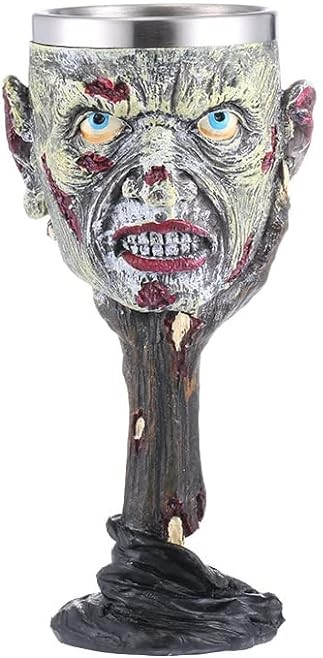
\includegraphics[width=0.23\textwidth]{kuvat/viinipikari_hirvio.jpg}
    \caption*{Vanhat pikarit}
    \medskip
    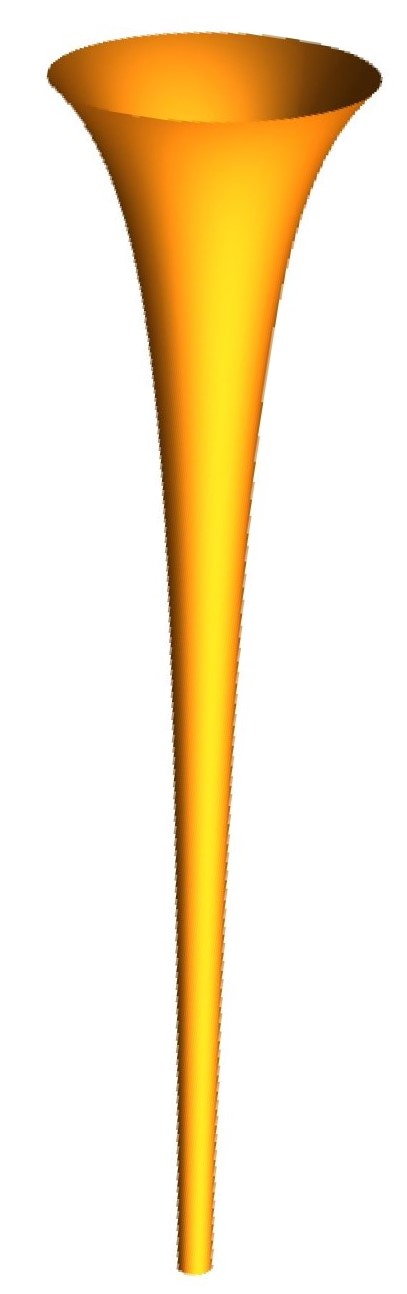
\includegraphics[width=0.23\textwidth]{kuvat/gabrielin_torvi.jpeg}
    \caption*{Torricellin idea uudeksi pikariksi}
    \end{center}
\end{wrapfigure}

Titanit Gabriel ja Torricelli istuivat titaanien baarissa tulivuori Vesuviuksen juurella. Gabriel ei pitänyt baarin viinipikareista. Ne olivat hänen mielestään liian epämääräisen muotoiset. Hän ei myöskään pitänyt pikarien väristä. Gabriel halusi pikarin, joka on päällystetty kultaisella maalilla ja on geometrisen muotoinen.

Torricelli ehdotti Gabrielille pikaria, joka on muodostettu käyrän $\frac{1}{x}$ pyörähdyspinnan osasta $x \ge 1$.

\begin{enumerate}
\item Pystyykö pikarin ulkopuolen maalaamaan realistisesti kultaisella maalilla?
\item Pystyykö pikarin täyttämään viinillä piripintaan?
\end{enumerate}

Vihje 1: Laske paljonko viiniä ja maalia tarvittaisiin.


Vihje 2: Pyörähdyskappaleen pinta-alalle ja tilavuudelle löytyy kaavat MAOLista.